\documentclass[12pt, a4paper]{report}
\usepackage{graphicx} %LaTeX package to import graphics
\usepackage[shortlabels]{enumitem}
\usepackage{geometry}
\geometry{lmargin=30mm}
\usepackage[export]{adjustbox}
\usepackage{titlesec}
\titleformat{\chapter}{\normalfont\huge}{\thechapter}{20pt}{\huge\bf}
\graphicspath{{images/}} %configuring the graphicx package
\title{Practica 1}
\author{Javier Izquierdo Hernández}
\date{\today}
\begin{document}
	\begin{titlepage}
		\centering
		{
\includegraphics[width=0.3\textwidth]{logo}\par}
		\vspace{1cm}
		{\bfseries\LARGE Universidad Rey Juan Carlos \par}
		\vspace{1cm}
		{\scshape\Large E.T.S. Ingeniería de Telecomunicación \par}
		\vspace{3cm}
		{\scshape\Huge Redes de Ordenadores para Robots y Máquinas Inteligentes \par}
		\vspace{3cm}
		{\itshape\Large Práctica 1 \par}
		\vfill
		{\Large Autor: \par}
		{\Large Javier Izquierdo Hernández \par}
		\vfill
		{\Large \today \par}
	\end{titlepage}

\newpage
\renewcommand{\contentsname}{Contenidos}
\tableofcontents
\newpage

\chapter{Funcionamiento básico de IPv6}
Para la realización de los siguientes ejercicios es necesario descomprimir el fichero IPv6-lab.tgz
que descargarás de la siguiente página:
\begin{center}
https://mobiquo.gsyc.urjc.es/practicas/ror/p1.html\\	
\end{center}
Al descomprimir este fichero se generará un directorio IPv6-lab con los archivos de configuración
de esta práctica necesarios para NetGUI.\\

Al arrancar NetGUI, debes abrir el escenario definido dentro del directorio IPv6-lab. Este
escenario es el que se muestra en la figura 1.
\section{Autoconfiguración de direcciones IPv6 \textit{(link-local)}}
\begin{figure}[h]
	\centering
	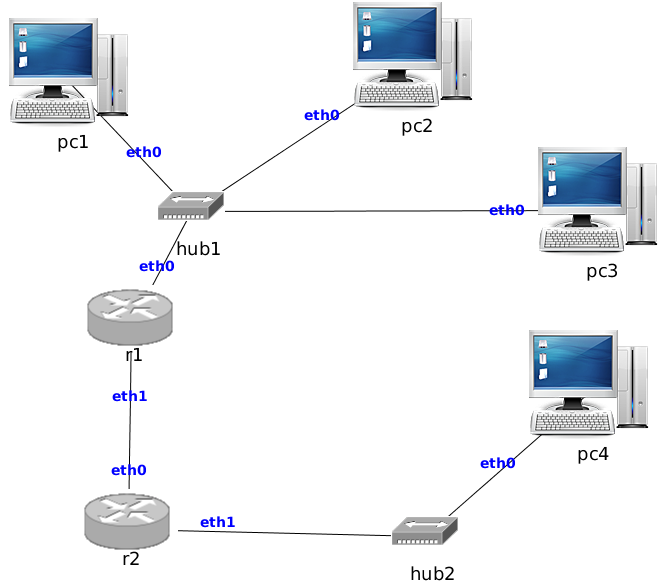
\includegraphics[width=0.7\textwidth]{fig1}
	\caption{Escenario de IPv6}
\end{figure}
Para empezar arranca únicamente pc1.\\
\begin{enumerate}
	\item Indica cuál es la dirección IPv6 link-local que se ha configurado en pc1, y su relación con su
	dirección Ethernet.\\	
	\begin{itemize}
		\item Dirección IPv6 link-local: fe80::214:23ff:feaa:d111/64
		\item Ethernet: 00:14:23:aa:d1:11
	\end{itemize}
	El 00 se convierte en 02, luego se añaden los 4 siguientes bytes 14 23. Luego en la dirección ip se añade ff fe y por último los 6 últimos bytes aa d1 11.
	\item Indica a qué dirección IPv6 multicast de nodo solicitado pertenece pc1.\\
	ff02::1:ffaa:d111
\end{enumerate}
Arranca tcpdump en pc1 para que capture paquetes y guarda la captura en el fichero ipv6-01.cap.
Arranca pc2.\\
\begin{enumerate}
	\setcounter{enumi}{2}
	\item Indica cuál es la dirección IPv6 link-local que se ha configurado en pc2, y su relación con su
	dirección Ethernet.\\
	\begin{itemize}
		\item Dirección IPv6 link-local: fe80::214:23ff:feaa:d122/64
		\item Ethernet: 00:14:23:aa:d1:22
	\end{itemize}
	El 00 se convierte en 02, luego se añaden los 4 siguientes bytes 14 23. Luego en la dirección ip se añade ff fe y por último los 6 últimos bytes aa d1 22.
	\item Indica a qué dirección IPv6 multicast de nodo solicitado pertenece pc2.\\
	ff02::1:ffaa:d122
	\item Interrumpe la captura que estabas realizando en pc1. Carga la captura en wireshark y localiza
	el mensaje enviado por pc2 que indica que pc2 está detectando si existen direcciones IPv6
	duplicadas con su dirección link-local.
	\begin{center}
		
\includegraphics[width=1\textwidth]{ej5_1_1}
	\end{center}
	\item Fíjate en las direcciones IPv6 y en las direcciones Ethernet que lleva este mensaje. Explica si
	la máquina pc1 recibe y procesa ese mensaje (aunque no responda).\\
	
	No responde ni procesa el mensaje ya que la dirección Ethernet de destino es 33:33:ff:aa:d1:22 que no corresponde con la dirección Ethernet multicast de pc1.
	\item Localiza los mensajes ICMPv6 Multicast Listener Report e indica cuál crees que es su propósito.
\begin{center}
		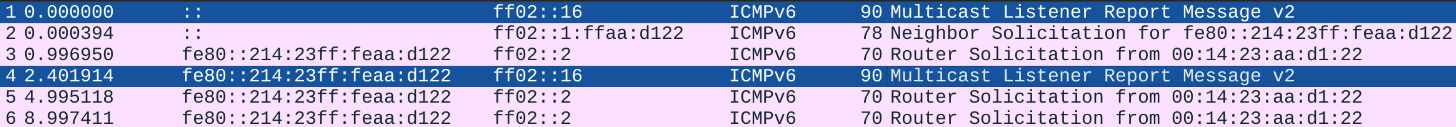
\includegraphics[width=1\textwidth]{ej7_1_1}
\end{center}
	\item Explica los mensajes ICMPv6 Router Solicitation que observas en la captura y explica su
	contenido y su propósito.\\
	
	El pc2 intenta encontrar un router para conseguir su dirección ipv6 global y como no hay uno encendido pc2 seguirá enviando mensajes a la dirección multicast de todos los routers.
\begin{center}
		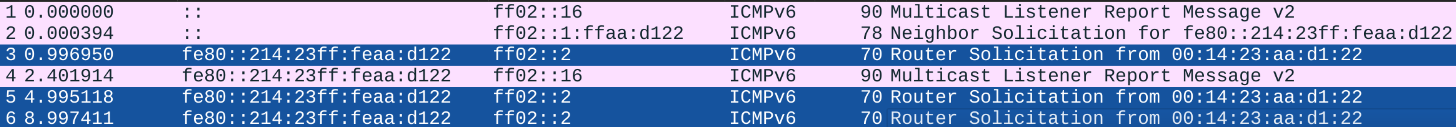
\includegraphics[width=1\textwidth]{ej8_1_1}
\end{center}
\end{enumerate}

Arranca tcpdump en pc1 para que capture paquetes y guarda la captura en el fichero ipv6-02.cap.
Arranca pc3.
\begin{enumerate}
	\setcounter{enumi}{8}
	\item Indica cuál es la dirección IPv6 link-local que se ha configurado en pc3, y su relación con su
	dirección Ethernet.
		\begin{itemize}
		\item Dirección IPv6 link-local: fe80::214:22ff:feaa:d122/64
		\item Ethernet: 00:14:22:aa:d1:22
	\end{itemize}
	El 00 se convierte en 02, luego se añaden los 4 siguientes bytes 14 22. Luego en la dirección ip se añade ff fe y por último los 6 últimos bytes aa d1 22.
	\item Indica a qué dirección IPv6 multicast de nodo solicitado pertenece pc3.\\
	ff02::1:ffaa:d122
	\item Interrumpe la captura que estabas realizando en pc1. Carga la captura en wireshark y localiza
	el mensaje enviado por pc3 que indica que pc3 está detectando si existen direcciones IPv6
	duplicadas con su dirección link-local.
\begin{center}
		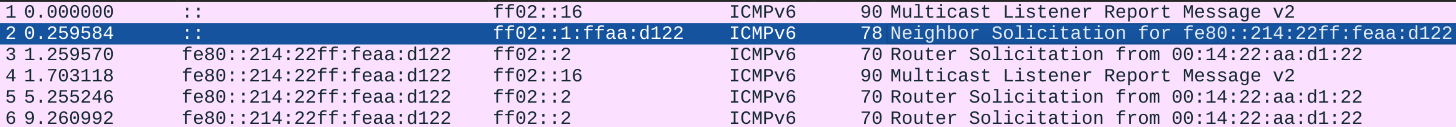
\includegraphics[width=1\textwidth]{ej11_1_1}
\end{center}
	\item Fíjate en las direcciones IPv6 y en las direcciones Ethernet que lleva este mensaje. Indica si
	las máquinas pc1 y/o pc2 reciben y procesan este mensaje (respondan o no).\\
	
	Si procesa el mensaje pc2 ya que la dirección Ethernet de destino es 33:33:ff:aa:d1:22 que se corresponde con la dirección Ethernet multicast de pc2. Y pc1 no recibe nada ya que su dirección Ethernet multicast es distinta.
	\item Observa en la captura si pc1 o pc2 responden al mensaje enviado por pc3, y explica por qué.\\
	
	No responde pc2 porque la dirección Ipv6 del mensaje de Neighbor Solicitation es fe80::214:23ff:feaa:d122 que es distinta de la de pc2 que es fe80::213:22ff:feaa:d122.
\end{enumerate}
\section{Tráfico IPv6 entre 2 máquinas directamente conectadas}
\begin{enumerate}
	\item Comprueba con el comando route las rutas IPv6 que tiene configuradas las máquinas pc1,
	pc2 y pc3 y explica el significado de las mismas.\\
	Los 3 ordenadores tienen las mismas rutas configuradas pero variando el numero de segundos de \textit{expire}.
	\begin{itemize}
		\item fe80::/64 dev eth0  metric 256  expires -2025sec mtu 1500 advmss 1440 hoplimit 4294967295
		\item ff00::/8 dev eth0  metric 256  expires -2025sec mtu 1500 advmss 1440 hoplimit 4294967295
	\end{itemize}
	\item Ejecuta tcpdump en pc3 (guardando los paquetes en un fichero ipv6-03.cap) y realiza un
	ping6 desde pc1 a la dirección link-local de pc2.
	\item Comprueba que funciona desde pc2 el ping6 a la dirección IPv6 multicast de nodo solicitado
	de pc1. Explica la respuesta que obtienes.\\
	
	Solo recibe una respuesta porque solo pc1 tiene esa dirección IPv6 multicast de nodo solicitado.
	\begin{center}
		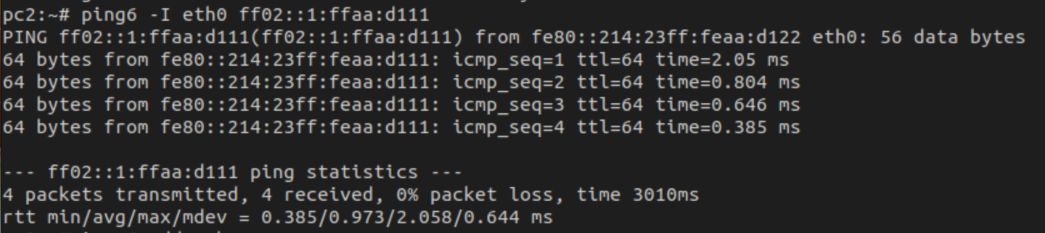
\includegraphics[width=1\textwidth]{ej3_1_2}
	\end{center}
	\item Comprueba que funciona desde pc1 el ping6 a la dirección IPv6 multicast de nodo solicitado
	de pc2. Explica la respuesta que obtienes.\\
	
	Recibe dos respuestas porque tanto pc2 como pc3 tienen la misma dirección IPv6 multicast de nodo solicitado.
	\begin{center}
		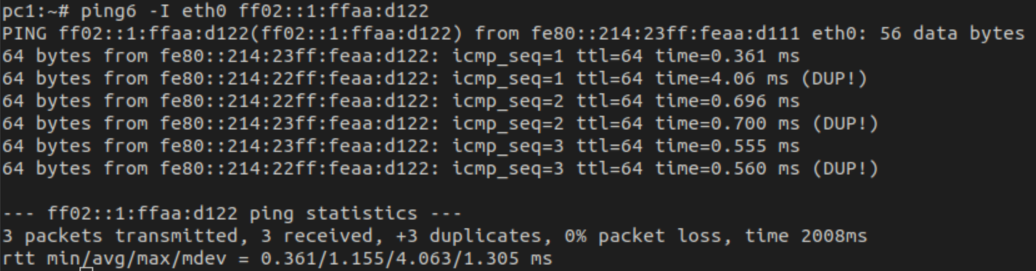
\includegraphics[width=1\textwidth]{ej4_1_2}
	\end{center}
	\item Comprueba que funciona desde pc1 el ping6 a la dirección IPv6 multicast de todos los nodos
	del enlace. Explica la respuesta que obtienes.\\
	
	Recibe tres respuestas porque manda el ping a todos los nodos, es decir a pc1, pc2 y pc3.
	\begin{center}
		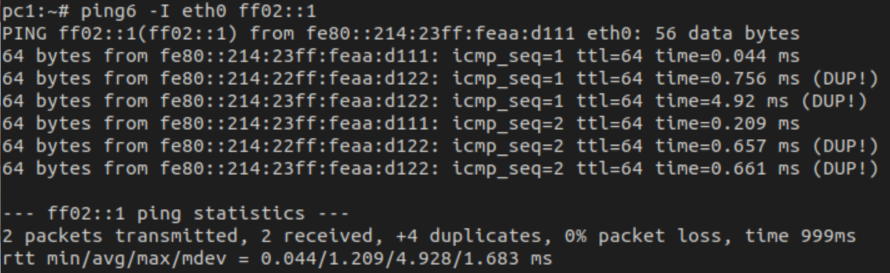
\includegraphics[width=1\textwidth]{ej5_1_2}
	\end{center}
	\item Interrumpe la captura.
	\item Localiza en la captura todos los mensajes de Neighbor Solicitation. Identifica en ellos qué máquina los envía, explica la causa por la que los envía. Fíjate en la dirección Ethernet de destino
	de dichos mensajes y explica su valor. ¿Qué máquinas recibirán cada uno de esos mensajes de
	\textit{Neighbor Solicitation}?
	\begin{itemize}
		\item Máquina de origen: pc1 ; Ethernet de destino: 00:14:23:aa:d1:22; Máquina de destino: pc2
		\item Máquina de origen: pc2 ; Ethernet de destino: 00:14:23:aa:d1:11; Máquina de destino: pc1
		\item Máquina de origen: pc3 ; Ethernet de destino: 33:33:ff:aa:d1:11; Máquina de destino: pc1
		\item Máquina de origen: pc1 ; Ethernet de destino: 00:14:22:aa:d1:22; Máquina de destino: pc3
		\item Máquina de origen: pc2 ; Ethernet de destino: 00:14:23:aa:d1:11; Máquina de destino: pc1
		\item Máquina de origen: pc1 ; Ethernet de destino: 00:14:23:aa:d1:22; Máquina de destino: pc2
	\end{itemize}
	Las direcciones Ethernet que empiezan por 00 son aquellas que los pc conocen para la dirección ipv6 de la máquina con la que quieren comunicarse, mientras que la qué es multicast (empieza por 33:33) será porque pc3 no conoze la dirección Ethernet real para pc1.
	\item Comprueba que tras la realización del ping6, las direcciones Ethernet de máquinas vecinas que
	han aprendido pc1 y pc2, mostrando la información de su caché de vecinos. Observa cuándo
	la información contenida cambia de estado y/o desaparece.\\
	
	NOTA: Ten en cuenta que la caché de vecinos de IPv6 en Linux tiene menor tiempo por defecto
	que la caché de ARP en IPv4. Prueba a utilizar watch -n 1 para repetir automáticamente el
	comando de consulta de la caché de vecinos, y repite el ping6 entre máquinas para ver mejor
	las transiciones entre estados.\\
	
	Primero las direcciones son DELAY, unos 5 segundos después pasa a REACHABLE, otros 15 segundos después pasa a STALE, y por último en más o menos un minuto sin actualizarse desaparecen.
\begin{center}
		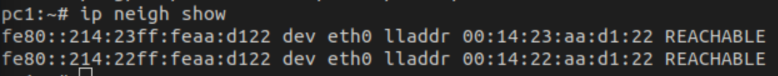
\includegraphics[width=1\textwidth]{ej8_1_1_2}
	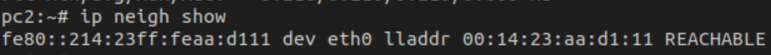
\includegraphics[width=1\textwidth]{ej8_2_1_2}
\end{center}
	\item Comprueba qué direcciones aprende pc3 en su caché de vecinos tras todo el tráfico anterior.\\
	
	Pc3 aprende la dirección de pc1.
\begin{center}
		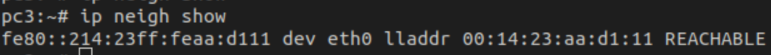
\includegraphics[width=1\textwidth]{ej9_1_2}
\end{center}
\end{enumerate}
\section{Autoconfiguración de direcciones IPv6 globales}
Arranca la máquina pc4, pero todavıía no arranques los routers r1 y r2.\\

Los routers r1 y r2 tienen configurado en el protocolo ICMPv6 el envío de mensajes Router
Advertisement. Nada más arrancar, estos routers mandan mensajes ICMPv6 Router Advertisement
que contienen anuncios de los prefijos de subred a los que pertenecen sus interfaces. De esta forma,
las máquinas que estén directamente conectadas a dichas interfaces podrán configurar su dirección
IPv6 en función de los anuncios que reciban.\\

Arranca (en background ) una captura en pc4 y guárdala en un fichero ipv6-04.cap.\\
\begin{enumerate}
	\item Indica qué direcciones y rutas ha configurado pc4.
	\begin{itemize}
		\item Dirección IPv6 link-local: fe80::214:23ff:feaa:d188/64
		\item Dirección Ipv6 Multicast: ff02::1:ffaa:d188
		\item Ethernet: 00:14:23:aa:d1:88
		\item Rutas:
		\begin{itemize}
			\item fe80::/64 dev eth0  metric 256  expires -253sec mtu 1500 advmss 1440 hoplimit 4294967295
			\item ff00::/8 dev eth0  metric 256  expires -253sec mtu 1500 advmss 1440 hoplimit 4294967295
		\end{itemize}
	\end{itemize}
\end{enumerate}
Arranca r2.
\begin{enumerate}
	\setcounter{enumi}{1}
	\item Indica qué direcciones y rutas tiene ahora configuradas pc4.
	\begin{itemize}
		\item Dirección IPv6 link-local: fe80::214:23ff:feaa:d188/64
		\item Dirección IPv6 link-global: 2001:db8:300:300:214:23ff:feaa:d188/64
		\item Dirección Ipv6 Multicast: ff02::1:ffaa:d188
		\item Ethernet: 00:14:23:aa:d1:88
		\item Rutas:
		\begin{itemize}
			\item 2001:db8:300:300::/64 dev eth0  proto kernel  metric 256  expires 57sec mtu 1500 advmss 1440 hoplimit 4294967295
			\item fe80::/64 dev eth0  metric 256  expires -362sec mtu 1500 advmss 1440 hoplimit 4294967295
			\item ff00::/8 dev eth0  metric 256  expires -362sec mtu 1500 advmss 1440 hoplimit 4294967295
			\item default via fe80::214:23ff:feaa:d177 dev eth0  proto kernel  metric 1024  expires 27sec mtu 1500 advmss 1440 hoplimit 64
			
		\end{itemize}
	\end{itemize}
	\item Interrumpe la captura en pc4 y explica los mensajes que observas en dicha captura. Fíjate en
	las direcciones IPv6 origen y destino de cada paquete. Explica el sentido del último mensaje
	que aparece en la captura que NO es un Router Advertisement.\\
	
	Los mensajes de la captura se pueden dividir en 3 partes, en la primera r2 se asigna una dirección ipv6 local, en la segunda una global y por último empieza a asignar direcciones ipv6 globales a todos los nodos conectados.\\
	En el último mensaje el router r2 se autoconfigura la ipv6 global enviandose un Neighbor solicitation a si mismo para esa ip.
	\item Muestra las direcciones de vecinos aprendidas por r2 y pc4 y justifica tu respuesta.\\
	
	R2 no aprende ninguna dirección, ya que no ha recibido ningún mensaje, mientras que pc4 tiene aprendida la dirección del router pero esta en STALE porque no ha confirmado la dirección.
\begin{center}
		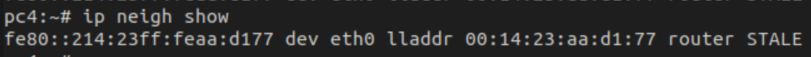
\includegraphics[width=1\textwidth]{ej4_2_1_3}
\end{center}
	\item  Indica los valores Valid Lifetime (valid lft) y Preferred Lifetime (preferred lft) de la dirección
	IPv6 global que se ha configurado en pc4. ¿De dónde los ha tomado pc4?. Relaciona estos
	valores con los intervalos entre mensajes Router Advertisement que se ven en la captura.\\
	
	El valor de Valid Lifetime y de Preferred Lifetime los toma del router que le da la dirección IPv6 global, y estos son 64 y 32 respectivamente.
	El intervalo de los Router Advertisement es de 4.5 segundos, y se puede apreciar que los valores anteriores se reinician cada aprox. 5 segundos, que es más o menos lo mismo que el intervalo.
	\item Interrumpe la ejecución del demonio radvd en r2.\\
	
	Indica qué ocurre con los valores valid lft y preferred lft. en pc4. Indica también qué ocurre
	con la dirección IPv6 global que se había configurado en pc4, y en cuánto tiempo. Muestra las
	direcciones de vecinos aprendidas por pc4 y justifica tu respuesta.\\
	
	Ya no se restea el timer y al llegar a 60 seg se olvida como se puede apreciar en las siguentes imágenes.
\begin{center}
		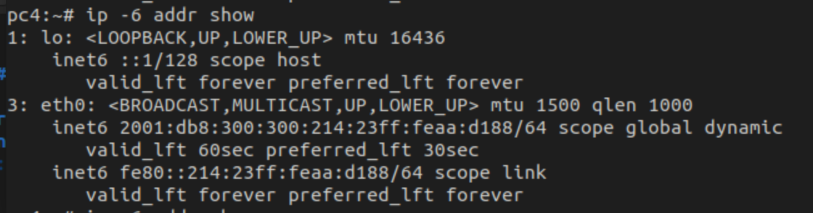
\includegraphics[width=1\textwidth]{ej6_1_1_3}\\
	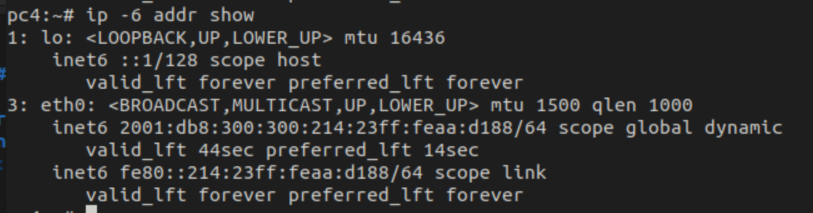
\includegraphics[width=1\textwidth]{ej6_2_1_3}\\
	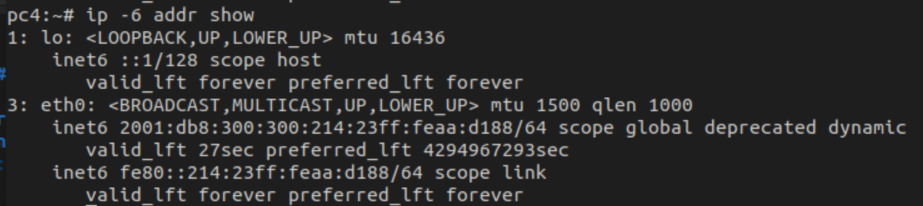
\includegraphics[width=1\textwidth]{ej6_3_1_3}\\
	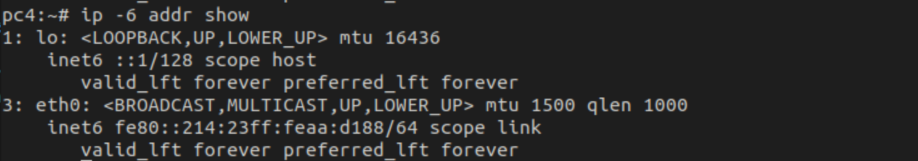
\includegraphics[width=1\textwidth]{ej6_4_1_3}\\
\end{center}
	Esto resulta en que las direcciones de vecinos desaparecen.
\begin{center}
		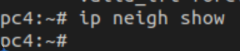
\includegraphics[width=0.3\textwidth]{ej6_5_1_3}
\end{center}
\end{enumerate}

Inicia en r2 el protocolo Router Advertisement y arranca r1.
\begin{enumerate}
	\setcounter{enumi}{6}
	\item Indica qué direcciones IPv6 globales se han configurado en pc1, pc2 y pc3.
	\begin{itemize}
		\item Pc1: 2001:db8:100:100:214:23ff:feaa:d111
		\item Pc2: 2001:db8:100:100:214:23ff:feaa:d122
		\item Pc3: 2001:db8:100:100:214:22ff:feaa:d122
	\end{itemize}
	\item Indica qué rutas IPv6 se han configurado en pc1, pc2 y pc3. Ejecuta repetidas veces en uno
	de los pcs el comando que visualiza las rutas y fíjate en lo que ocurre con el campo expires y
	trata de explicarlo. ¿De donde toma el pc ese valor?\\
	
	Cuando expire el valid\_lft perderá la IPv6 global, ya que no sabe si esta es válida para comunicarse son otras redes, ya que el router que le conecta con el exterior no se lo ha confirmado. El pc toma ese valor del router, y este es generado a partir de la dirección Ethernet.\\
	
	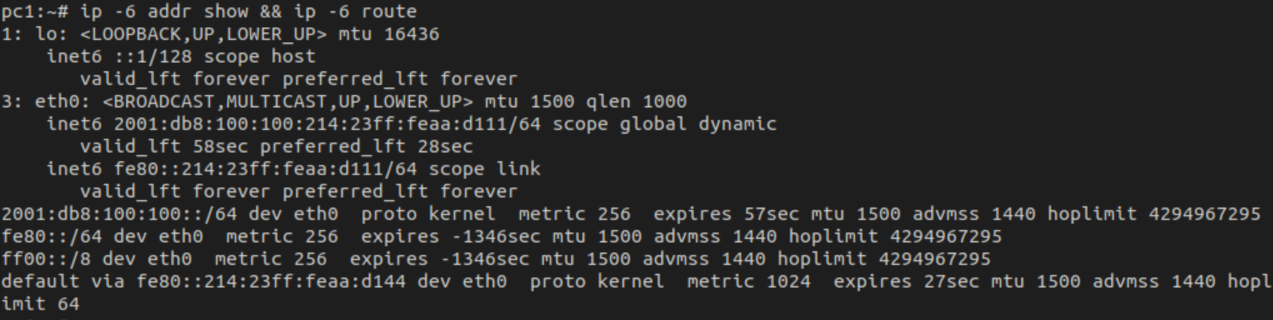
\includegraphics[width=1\textwidth]{ej8_1_1_3}\\
	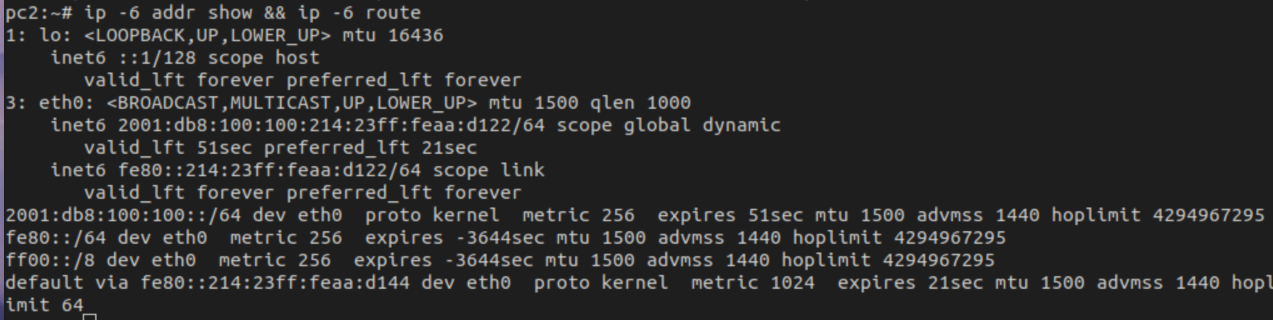
\includegraphics[width=1\textwidth]{ej8_2_1_3}\\
	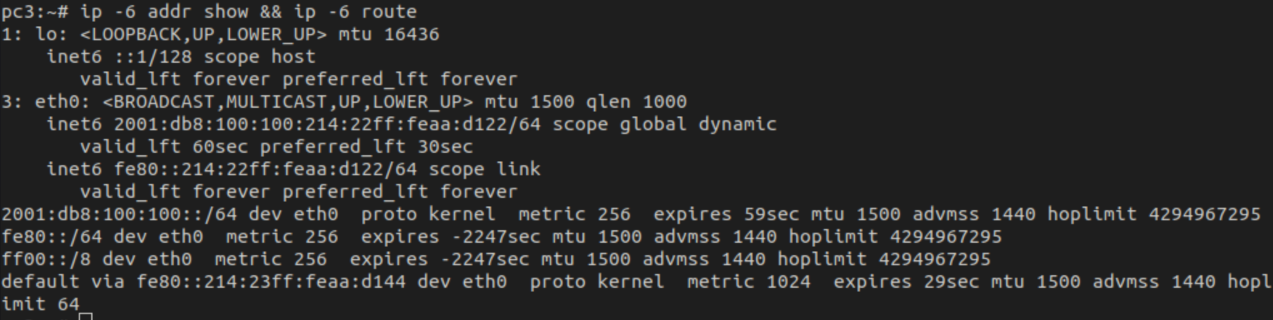
\includegraphics[width=1\textwidth]{ej8_3_1_3}
	\item Explica qué ocurre si haces un ping6 entre dos máquinas que no están directamente conectadas,
	por ejemplo, pc1 y pc4, o entre pc1 y r2. Para entenderlo consulta las rutas en las máquinas,
	y haz capturas en las interfaces que necesites.\\
	
	Si se hace ping desde pc1 a pc4 o a r2 no se consigue respuesta, porque r1 no tiene una ruta puesta para 2001:db8:300:300 y que r2 no tiene una ruta para 2001:db8:100:100.\\
	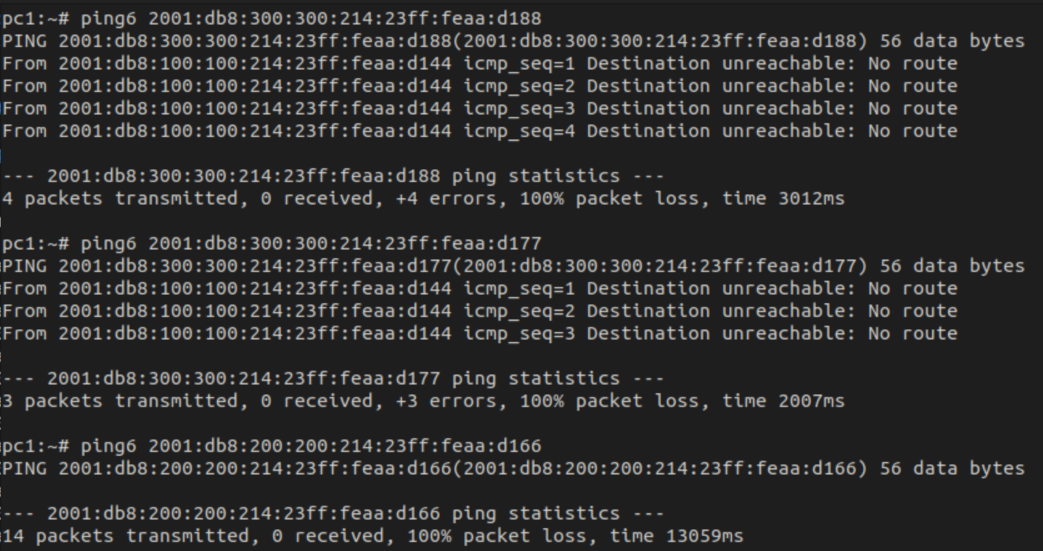
\includegraphics[width=1\textwidth]{ej9_1_3}
	\item Haz un ping desde pc1 a la IPv6 destino ff02::2. ¿Quién responde? Justifica la respuesta.\\
	
	Solo responde r1, ya que r2 no tiene una ruta configurada para responder a pc1 como he explicado anteriormente.
\end{enumerate}
\section{IPv6 entre 2 máquinas de subredes diferentes}
Los pcs tienen configuradas rutas por defecto, pero los routers sólo tienen configurada ruta hacia
máquinas vecinas. Como habrás comprobado en el apartado anterior, para que las máquinas de
diferentes subredes puedan intercambiar tráfico es necesario añadir rutas en los routers.
\begin{enumerate}
	\item Añade las rutas que consideres necesarias para que todas las máquinas de la figura puedan
	intercambiar tráfico entre ellas. Indica qué rutas has configurado.\\
	He añadido a r1 una ruta hacia 2001:db8:300:300::/64 via r2, y desde r2 una ruta hacia 2001:db8:100:100::/64 via r1.\\
	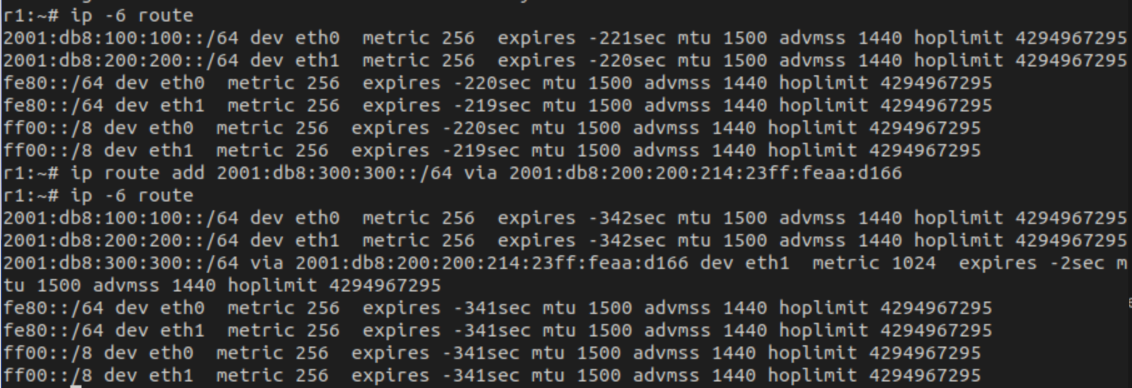
\includegraphics[width=1\textwidth]{ej1_1_2}
	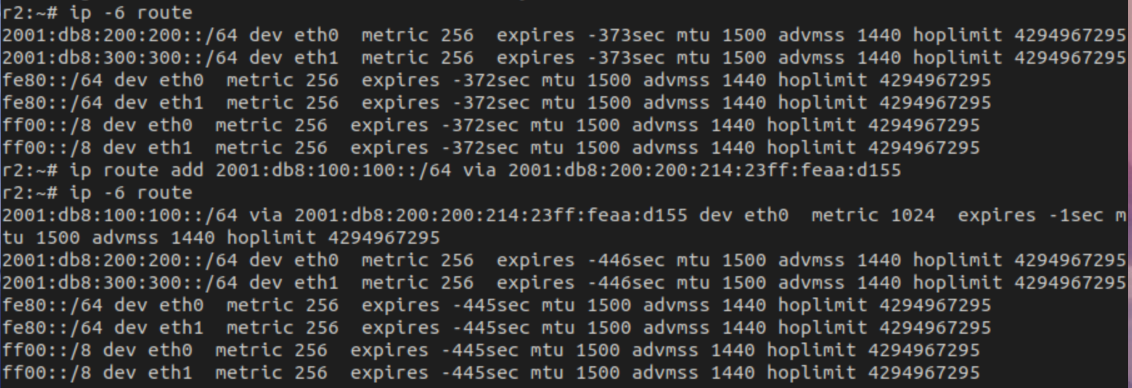
\includegraphics[width=1\textwidth]{ej1_2_2}
	\item Arranca un captura en alguna de las máquinas conectadas al hub1 y guárdala en un fichero
	ipv6-05.cap. Realiza un ping6 de pc1 a pc4 y otro de pc1 a la dirección global de la interfaz
	eth0 de r2. Interrumpe la captura y comprueba el fichero de captura. Observa las direcciones
	Ethernet e IP de los mensajes capturados, y el valor del hop limit.\\
	
	El hop limit solo varía en los Echo (ping), ya que en el resto siempre valen 255. En el primer ping el hop limit en el Echo request es 64 ya que pc1 está conectado al hub1 y en el reply es 62 porque tiene que pasar por 2 routers. En el segundo ping es igual salvo que en el reply solo pasa por un router, por lo tanto es 63.\\
	
	Luego en el resto de mensajes obviando los Router Advertisement y los Echo se puede ver que r1 pregunta a pc1 para confirmar su dirección ipv6 global.
	
\end{enumerate}
\chapter{Fragmentación en IPv6}
Para analizar la cabecera de extensión para la fragmentación en IPv6 vamos a provocar que sea
necesario fragmentar los datagramas IPv6.\\

En IPv6 sólo puede fragmentar la máquina que crea un datagrama y por tanto, no pueden fragmentar los routers intermedios que hay entre el origen y el destino (en IPv4 los routers intermedios
sí pueden fragmentar). NOTA: Ten en cuenta que los tamaños de los fragmentos de IPv6 deben ser
un múltiplo de 8 bytes, salvo el último (igual que en IPv4).\\

El valor de MTU por defecto en Ethernet es 1500 bytes (puedes comprobarlo con el comando
ip -6 addr).\\


Realiza una captura de tráfico en r1(eth0) (fichero ipv6-06.cap) y en r2(eth0) (fichero
ipv6-07.cap).\\

Ejecuta un ping6 desde pc1 a la dirección global de pc4 con la opción -s 2000 obligando a
que los paquetes de ICMPv6 echo request tengan 2000 bytes de datos, provocando un tamaño de
datagrama IPv6 mayor que la MTU de Ethernet.\\

Interrumpe las capturas y estúdialas.
\begin{enumerate}
	\item Explica qué máquina ha fragmentado los datagramas y cómo sabe a qué tamaño máximo debe
	hacerlo.\\
	
	Los ha fragmentado los pc que mandan y reciben el Echo, y los han fragmentado al tamaño por defecto de datagrama máximo en Ethernet que es 1500.
	\item Estudia los valores de las cabeceras Next Header cuando un datagrama se fragmenta, y trata
	de comprobar los tamaños de los fragmentos y el tamaño del datagrama original sin fragmentar
	que se quería enviar.\\
	
	El valor de la cabecera Next Header cambia si tiene más fragmentos, esto se ve en el flag de More Fragments. Esta cabecer tiene un tamaño de 44 bits, con lo que al unirlo con el tamaño del primer datagrama obtenemos 1500, lo que es el máximo.\\
	Y por último, para encontrar el tamaño original del datagrama solo sumamos las 2 partes y el resultado es 2024 bits.
\end{enumerate}

Ahora vamos a modificar el valor de la MTU entre r1 y r2 para que sea 1304 bytes (en vez de
los 1500 tipos de Ethernet). Para ello ejecuta el siguiente comando en r1 para modificar el valor de
MTU en su interfaz eth1:\\

\textbf{r1:$\sim\#$ ip link set eth1 mtu 1304}\\

Y ejecuta el siguiente comando en r2 para modificar el valor de MTU en su interfaz eth0:\\

\textbf{r2:$\sim\#$ ip link set eth0 mtu 1304}\\

Realiza una captura de tráfico en r1(eth0) (fichero ipv6-08.cap) y en r2(eth0) (fichero
ipv6-09.cap). Ejecuta un ping6 desde pc1 a la dirección global de pc4 con la opción -s 1400.
Interrumpe las capturas y estúdialas.\\
\begin{enumerate}
	\setcounter{enumi}{2}
	\item Explica qué máquina ha fragmentado los datagramas y cómo sabe a qué tamaño debe hacerlo.
	Trata de comprobar los tamaños de los fragmentos y el tamaño del datagrama original sin
	fragmentar que se quería enviar.\\
	
	La máquina que fragmenta los datagramas es pc1. Primero envía el datagrama ip de 1408 bits de tamaño a lo que r1 responde con un mensaje diciendo a pc1 que el tamaño máximo es 1304, con lo que pc1 reenvía el mensaje fragmentándolo de manera adecuada.
	\item Explica la diferencia que ves entre los 2 ficheros de capturas.\\
	
	Entre la captura 6 y la 8 la diferencia está en el mensaje que envía r1 a pc1 diciéndole que el datagrama es demasiado grande y que el tamaño máximo es 1304.
\end{enumerate}
\chapter{Túnel IPv6 in IPv4}
Descomprime el laboratorio IPv6-tun-lab.tgz y carga el escenario dentro de NetGUI. Arranca
de una en una todas las máquinas del escenario.\\
Observa en la figura 2 que hay 3 zonas diferenciadas en el escenario:
\begin{itemize}
	\item Zona A - Zona IPv6: pc1, pc2 y r1.
	\item Zona B - Zona IPv4: r3, r4 y r5
	\item Zona C - Zona IPv6: r7, pc3 y pc4.
\end{itemize}
\begin{figure}[h]
	\centering
	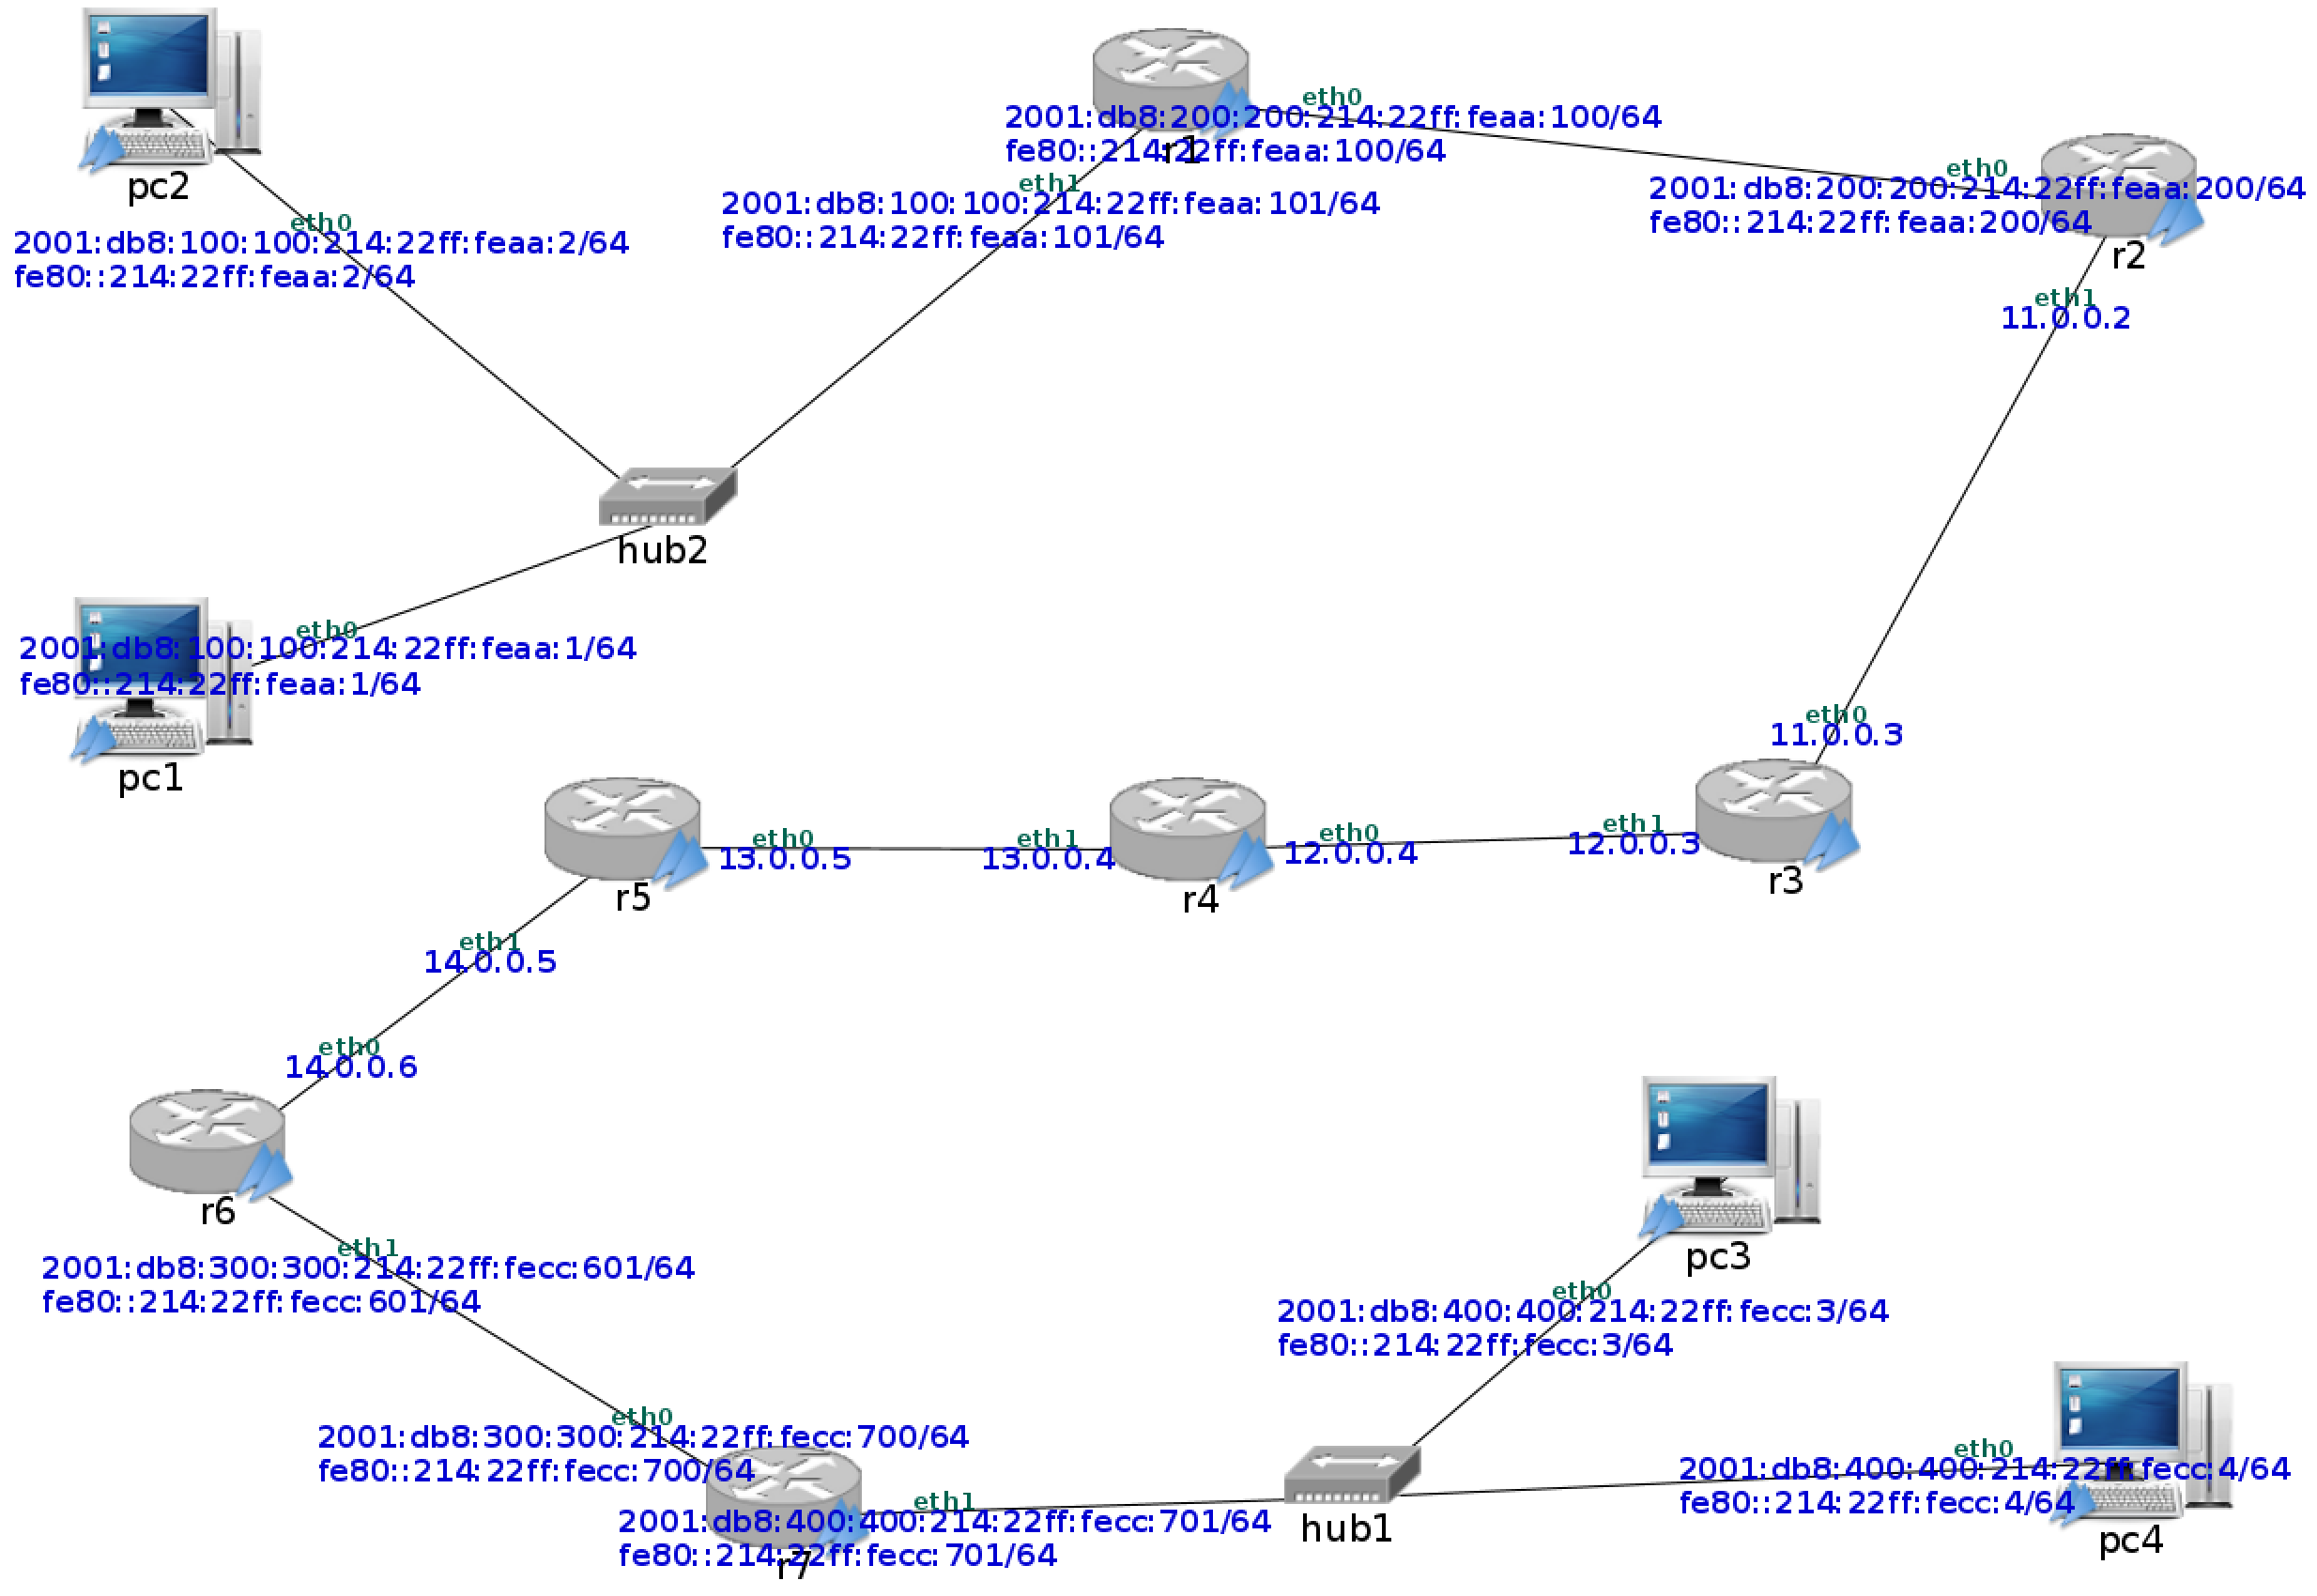
\includegraphics[width=1\textwidth]{fig2}
	\caption{Zonas IPv6 a través de una zona IPv4}
\end{figure}
Para empezar 
Los routers r2 y r6 son routers que interconectan zonas diferentes. Estos routers se comunican
por IPv4 en una de sus interfaces y por IPv6 en la otra. Son routers frontera que tienen la doble pila
(IPv4 e IPv6) instalada. Las máquinas r4 y r5 sólo se comunican por IPv4, y el resto de máquinas
(pc1, pc2, r1, r2, r7, pc3 y pc4) sólo se comunican por IPv6.\\

Todos los routers y máquinas tienen configuradas direcciones IP y rutas válidas para comunicarse
con los nodos de su misma zona.\\

Si haces ping6 desde pc1 a pc3 observarás que no funciona. Ambas máquinas están utilizando
IPv6, sin embargo, tienen que atravesar una zona que sólo está utilizando IPv4.\\

Para solucionar este problema vamos a configurar un Túnel IP punto a punto, metiendo los
paquetes IPv6 que se generen en ambas zonas IPv6 dentro de paquetes IPv4. De esta forma, las
máquinas IPv6 de diferentes zonas podrán comunicarse.\\
\begin{enumerate}
	\item Indica qué routers crees que deberían ser los extremos del túnel IPv6 dentro de IPv4.\\
	
	Los routers en los extremos deberían ser r2 y r6.
	\item Configura en r2 un extremo del túnel, con ttl 32, y añade la/s ruta/s necesaria/s en r2 para
	que los paquetes IPv6 generados en la zona A puedan llegar a la Zona C.
	\item Arranca 3 tcpdump:
	\begin{itemize}
		\item tcpdump en la interfaz eth1 de r1 (captura ipv6-tun-01.cap).
		\item tcpdump en la interfaz eth1 de r4 (captura ipv6-tun-02.cap).
		\item tcpdump en la interfaz eth1 de r7 (captura ipv6-tun-03.cap).
	\end{itemize}
	Realiza un ping6 desde pc1 a pc3. Verás que no funciona, pues aún no está configurado el
	otro extremo del túnel. Interrumpe las capturas y estúdialas.\\
	Con la configuración actual ¿llegan a viajar los ICMPv6 echo request por el túnel? Estudia las
	cabeceras exactas que llevan y explica sus valores.\\
	
	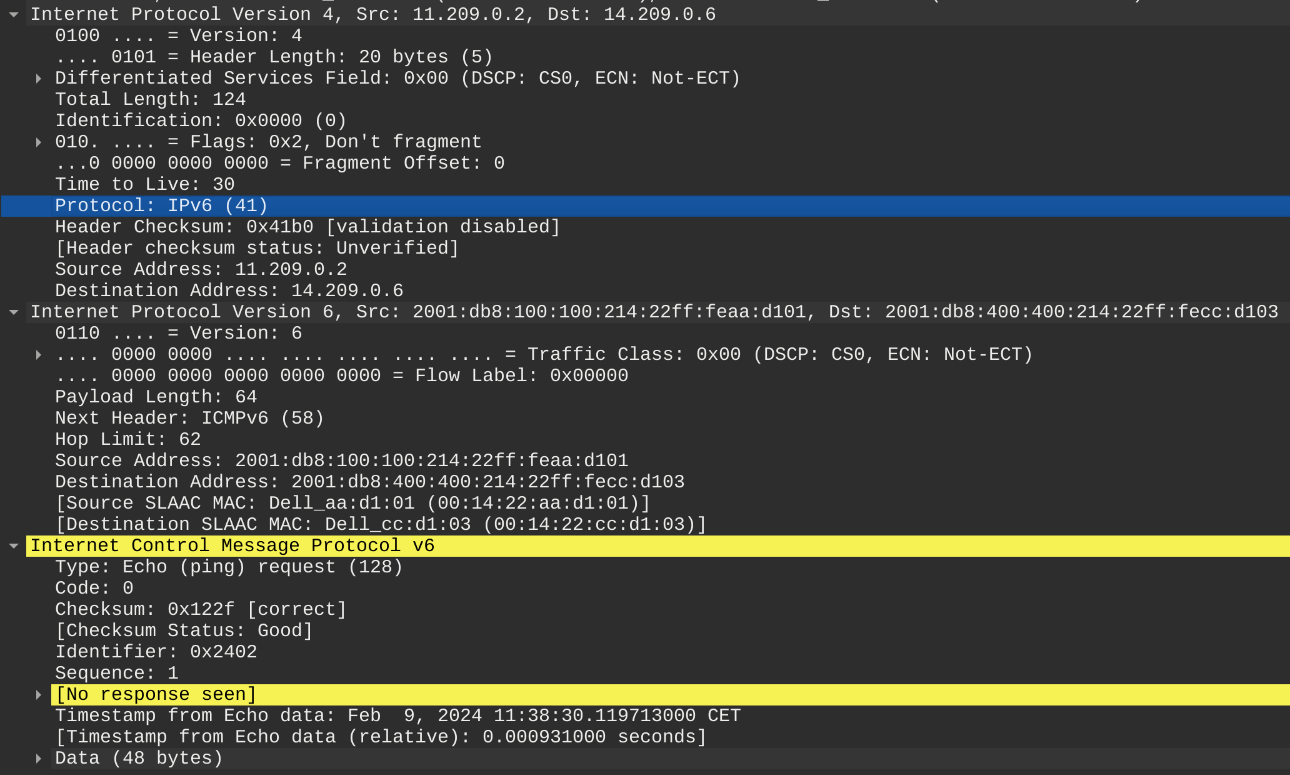
\includegraphics[width=1\textwidth]{ej3_3}\\
	
	Los mensajes viajan por el túnel hasta r6, donde al no estar configurado da error y envía de vuelta a r2 un datagrama ICMP con Protocol Unreachable.\\
	En las cabeceras de los Echo request se puede ver una exterior de IPv4 con el protocolo 41 diciendo que su contenido es IPv6, y dentro el datagrama original de IPv6.
	\item Configura en r6 el otro extremo del túnel, con ttl 32 y añade la/s ruta/s necesaria/s en r6
	para que los paquetes IPv6 generados en la zona C puedan llegar a la Zona A.
	\item Arranca 3 tcpdump:
	\begin{itemize}
		\item tcpdump en la interfaz eth1 de r1 (captura ipv6-tun-04.cap).
		\item tcpdump en la interfaz eth1 de r4 (captura ipv6-tun-05.cap).
		\item tcpdump en la interfaz eth1 de r7 (captura ipv6-tun-06.cap).
	\end{itemize}
	Realiza de un ping6 desde pc1 a pc3. Interrumpe las capturas y analízalas. Para los paquetes
	de cada una de las capturas, observa los siguientes campos y explica sus valores:
	\begin{enumerate}[a)]
		\item Versión del protocolo IP que hay en la cabecera IP que va justo detrás de la cabecera
		Ethernet.
		\item direcciones IP origen y destino de esa cabecera
		\item TTL (IPv4) o Hop limit (IPv6)
		\item Protocol (IPv4) o Next Header (IPv6)
		\item Contenido del datagrama IPv4 o IPv6.
	\end{enumerate}
	Solo estudio los Echo request y Echo reply:
	\begin{itemize}
		\item En r1: Echo request
		\begin{enumerate}[a)]
			\item IPv6
			\item Origen: 2001:db8:100:100:214:22ff:feaa:d101\\
			Destino: 2001:db8:400:400:214:22ff:fecc:d103
			\item 64 (porque pc1 está conectado a r1)
			\item ICMPv6 (para el ping)
			\item Echo (ping) request
		\end{enumerate}
		Como r1 está fuera del túnel solo tendrá IPv6.
		\item En r1: Echo reply
		\begin{enumerate}[a)]
			\item IPv6
			\item Origen: 2001:db8:400:400:214:22ff:fecc:d103\\
			Destino: 2001:db8:100:100:214:22ff:feaa:d101
			\item 60 (porque pasa por r7, r6, r2 y r1 (eth0))
			\item ICMPv6 (para el ping)
			\item Echo (ping) reply
		\end{enumerate}
		Como r1 está fuera del túnel solo tendrá IPv6, y para el Hop limit hay que tener en cuenta que el túnel no lo modifica.
		\item En r4: Echo request
		\begin{enumerate}[a)]
			\item IPv4
			\item Origen: 11.209.0.2\\
			Destino: 14.209.0.6
			\item 30 (pasa por r3 y por r4(eth0))
			\item IPv6 (porque encapsula el datagrama original)
			\item Echo (ping) request
		\end{enumerate}
		Como r4 está en el túnel tendrá IPv4 y dentro IPv6. También el origen del datagrama será r2 y el destino r6.
		\item En r4: Echo reply
		\begin{enumerate}[a)]
			\item IPv4
			\item Origen: 14.209.0.6\\
			Destino: 11.209.0.2
			\item 31 (pasa por r5)
			\item IPv6 (porque encapsula el datagrama original)
			\item Echo (ping) reply
		\end{enumerate}
		Como r4 está en el túnel tendrá IPv4 y dentro IPv6. También el origen del datagrama será r6 y el destino r2.
		\item En r7: Echo request
		\begin{enumerate}[a)]
			\item IPv6
			\item Origen: 2001:db8:100:100:214:22ff:feaa:d101\\
			Destino: 2001:db8:400:400:214:22ff:fecc:d103
			\item 60 (porque pasa por r1, r2, r6 y r7 (eth0))
			\item ICMPv6 (para el ping)
			\item Echo (ping) request
		\end{enumerate}
		Como r7 está fuera del túnel solo tendrá IPv6.
		\item En r7: Echo reply
		\begin{enumerate}[a)]
			\item IPv6
			\item Origen: 2001:db8:400:400:214:22ff:fecc:d103\\
			Destino: 2001:db8:100:100:214:22ff:feaa:d101
			\item 64 (porque pc3 está conectado a r7)
			\item ICMPv6 (para el ping)
			\item Echo (ping) reply
		\end{enumerate}
		Como r7 está fuera del túnel solo tendrá IPv6, y para el Hop limit hay que tener en cuenta que el túnel no lo modifica.
	\end{itemize}
	Utiliza la herramienta traceroute6 para conocer el número de saltos IPv6 que se dan desde pc2
	a pc4. Esta herramienta tiene un comportamiento similar al traceroute en IPv4. Si no recuerdas
	su funcionamiento, por favor, revísalo antes de comenzar este apartado.\\
	IMPORTANTE: Para usar traceroute6 en este escenario, utiliza siempre la opción -z 200 para
	que traceroute6 espere 200ms entre cada paquete que envía.
	\item Piensa en qué paquetes se van a capturar en las interfaces r4(eth1), r1(eth1) y r7(eth1)
	cuando ejecutes traceroute6 desde pc2 a pc4.\\
	
	
	\item Inicia 3 capturas de tráfico:
	\begin{itemize}
		\item en la interfaz eth1 de r1 (captura ipv6-tun-07.cap).
		\item en la interfaz eth1 de r4 (captura ipv6-tun-08.cap).
		\item en la interfaz eth1 de r7 (captura ipv6-tun-09.cap).
	\end{itemize}
	y realiza traceroute -I 6 desde pc2 a pc4.
	\item Interrumpe las capturas y analiza el contenido de los paquetes capturados, observando especialmente los campos TTL (IPv4) o Hop limit (IPv6) de los paquetes.
	\begin{itemize}
		\item En r1: con Hop limit 1 cuando no ha entrado en el túnel, con 2 cuando entra en r2 y en el túnel, con 3 cuando llega a r6, con 4 cuando llega a r7 y al hub1 y con 5 al llegar a pc4.
		\item En r4: con Hop limit 1 cuando entra al túnel y con TTL 30 (es decir, 2 saltos), luego con Hop limit 2 al salir del túnel y con el mismo TTL, y por último con Hop limit 3 al llegar a pc4 (con TTL 30).
		\item En r7: solo hay con Hop limit 1.
	\end{itemize}
	\item Tras lo analizado en las capturas, explica con detalle cómo cambian los valores de Hop limit
	y TTL según los ICMPv6 echo request van avanzando por la zona A, después por la zona B, y
	por último por la zona C.\\
	
	Siguiendo con lo explicado en el apartado anterior se observa que:
	\begin{itemize}
		\item Zona A: el valor de Hop limit es el real, aumentando de manera constante por los routers que pasa excepto cuando esta en el túnel que no aumenta.
		\item Zona B: al estar dentro del túnel el valor del Hop limit se reinicia en r2 (la entrada al túnel) y el TTL será 32 - el número de routers que haya entre ese y r2.
		\item Zona C: el valor del Hop limit se vuelve a reiniciar en r6 (la salida del túnel).
	\end{itemize}
	\item Indica si ante el tráfico recibido por pc2, es posible que pc2 conozca que se ha atravesado un
	túnel para llegar a pc4.\\
	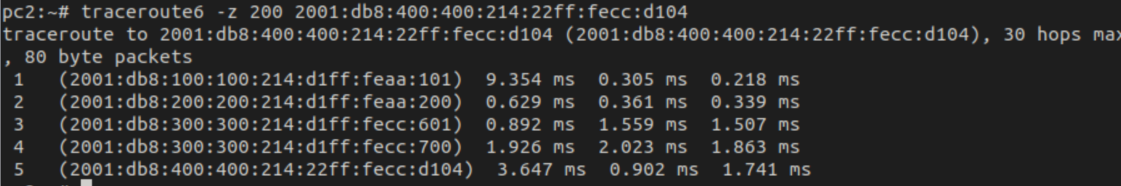
\includegraphics[width=1\textwidth]{ej10_3}
	No es posible que conozca que ha pasado por el túnel, ya que el Hop limit de la zona A no los tiene en cuenta.
\end{enumerate}
\end{document}
